\chapter{Charm Cascades}
The Charm Cascades allow you to browse the entire Anathema Charm database, consisting of the charms for the supported character types as well as those for the Dragon Kings. To open the Charm Cascades, either select the appropriate entry from the ``Extras'' menu or press their toolbar button.

An item tab will open, showing a large empty canvas and three combo boxes on top (see figure \ref{fig:CharmCascades}). Beginning from the right, they are used for selecting the Charm type shown (A), the charm tree to be displayed (B) and the edition and rule set whose data to use (C).

This last box, ruleset selection, should be set first, since changing editions forces the view to be reset. Intra-edition changes are made on the fly and take effect instantly, without reloading the charm tree.

Afterwards, select the Charm type you want to display, either one of the character types or ``Martial Arts'' for all the martial arts cascades available. Then, use the tree selection box to choose from the available trees.

Finally an image will load showing the structure of the charm cascade. By pointing your mouse on a Charm, a tooltip  (figure \ref{fig:CharmTooltip}) will be triggered. Within the tooltip, you will see everything there is to know about the charm\footnote{except for game effects, which are excluded due to copyright reasons}.

\begin{figure}[htbp]
	\centering
		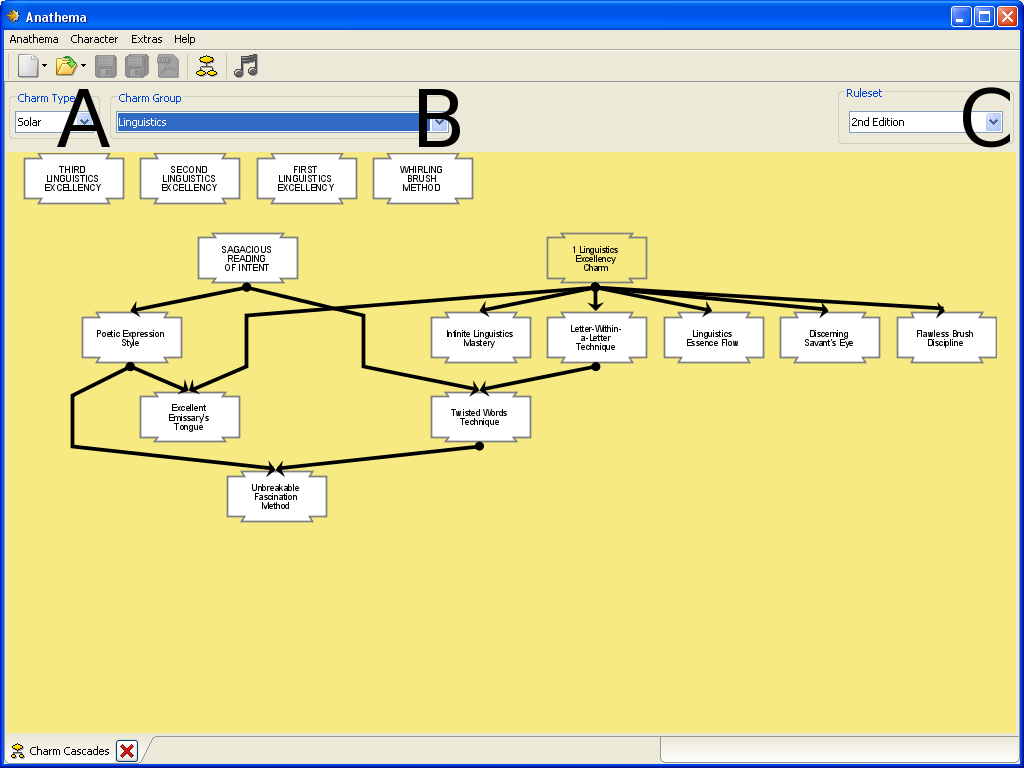
\includegraphics[width=1.00\textwidth]{images/CharmCascades.png}
	\caption{Charm Cascades}
	\label{fig:CharmCascades}
\end{figure}


\begin{figure}[htbp]
	\centering
		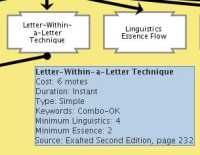
\includegraphics{images/CharmTooltip.jpg}
	\caption{Charm tooltip}
	\label{fig:CharmTooltip}
\end{figure}